\documentclass[12pt]{ufrslides}
\usepackage{textcomp}

\title[Projects]{My projects}
\author{E. Rasche}
\date{2017-11-09T08:00:00Z}
\newcommand{\ghpr}[3]{\href{https://github.com/#1/#2/pull/#3}{#1/#2\##3}}


\usepackage{siunitx}

\begin{document}
\frame{\titlepage}

\section[Completed]{Completed Projects}
\begin{frame}{Completed Projects}
	%Things that are \emph{completely} done and do not need updating
	%- galaxy hardening PR #4604
	%- 41% reduction in startup time https://github.com/galaxyproject/galaxy/pull/4495
	%- bigger click targets in Galaxy https://github.com/galaxyproject/galaxy/pull/4470
	%- LAN restrictions https://github.com/galaxyproject/galaxy/pull/4289
\end{frame}

\subsection[Monit/Infra]{Monitoring + Infrastructure}
	\begin{frame}{Initial Monitoring}
		\begin{center}
			\emph{New UFR Service}
		\end{center}
		\begin{itemize}
			\item Telegraf $\rightarrow$ InfluxDB $\rightarrow$ Grafana
			\item Open metrics / statistics
			\item Sharing dashboards with Galaxy project
			\item \url{https://grafana.denbi.uni-freiburg.de}
			% TODO: image
		\end{itemize}
	\end{frame}

	\begin{frame}{Sentry}
		\begin{center}
			\emph{New UFR Service}
		\end{center}
		\begin{itemize}
			\item Collects application exceptions
			\item Galaxy: stack traces, \texttt{log.warn}, \texttt{log.error}, \texttt{log.exception}
			\item Galaxy Frontend: javascript exceptions + browser info + user identity
			\item Helps catch + fix bugs!
		\end{itemize}
	\end{frame}


	{%
		\usebackgroundtemplate{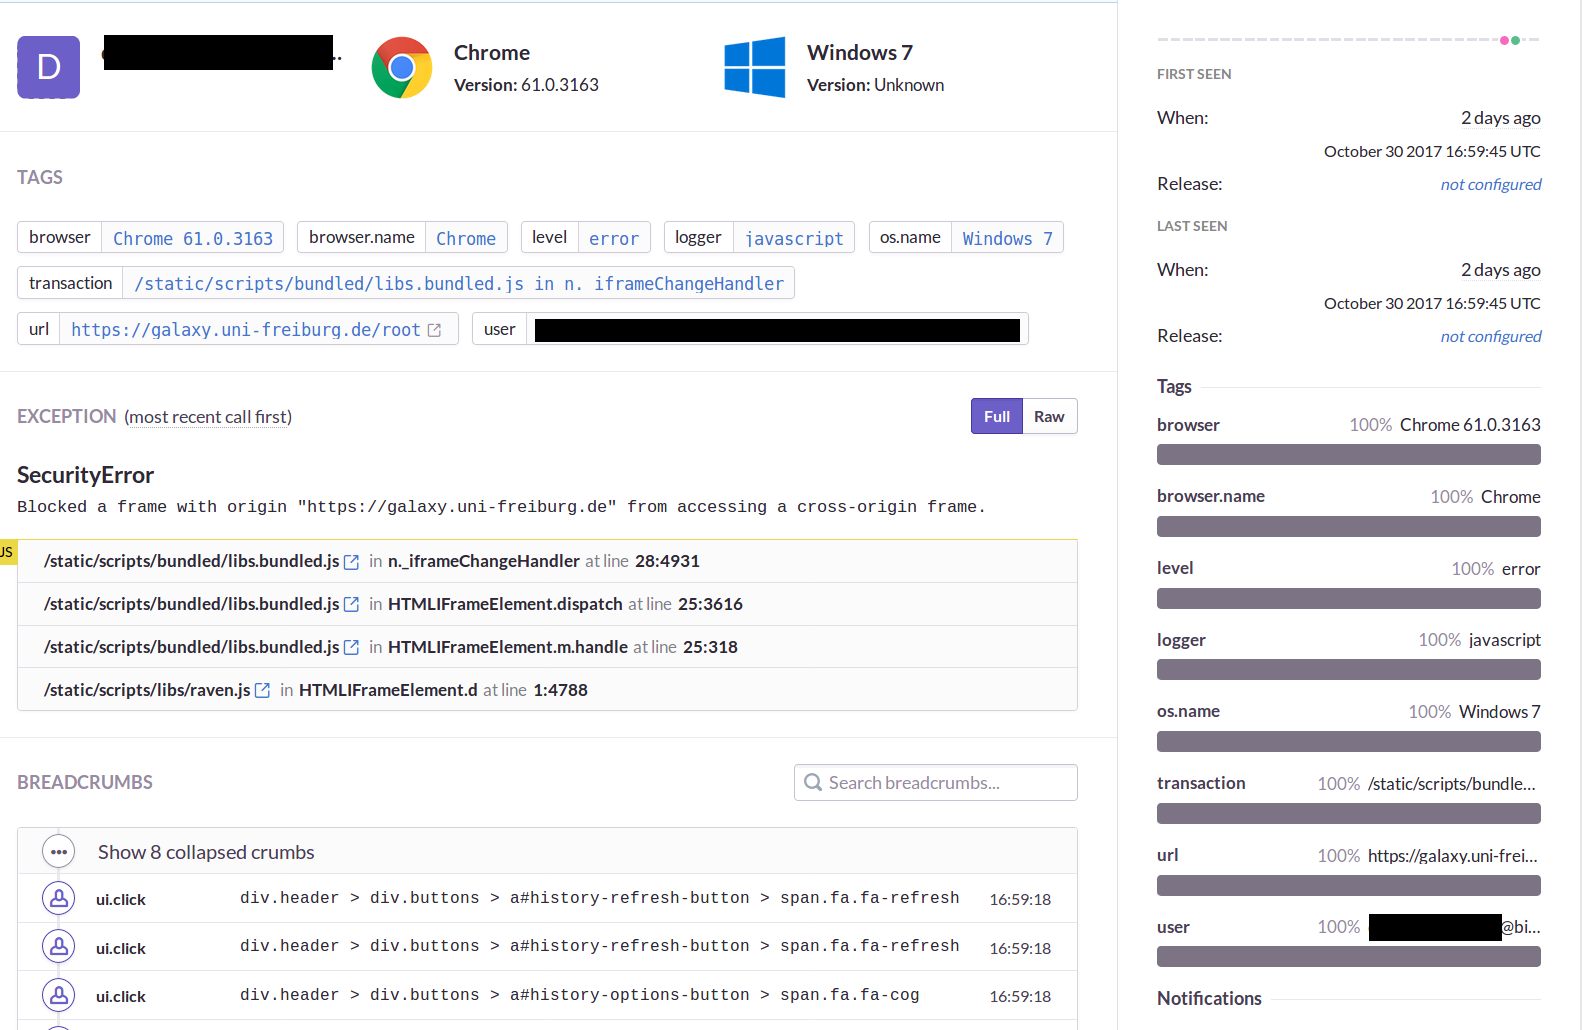
\includegraphics[height=\paperheight,width=\paperwidth]{sentry_1.png}}
		\setbeamertemplate{navigation symbols}{}
		\begin{frame}[plain]
		\end{frame}
	}

	{%
		\usebackgroundtemplate{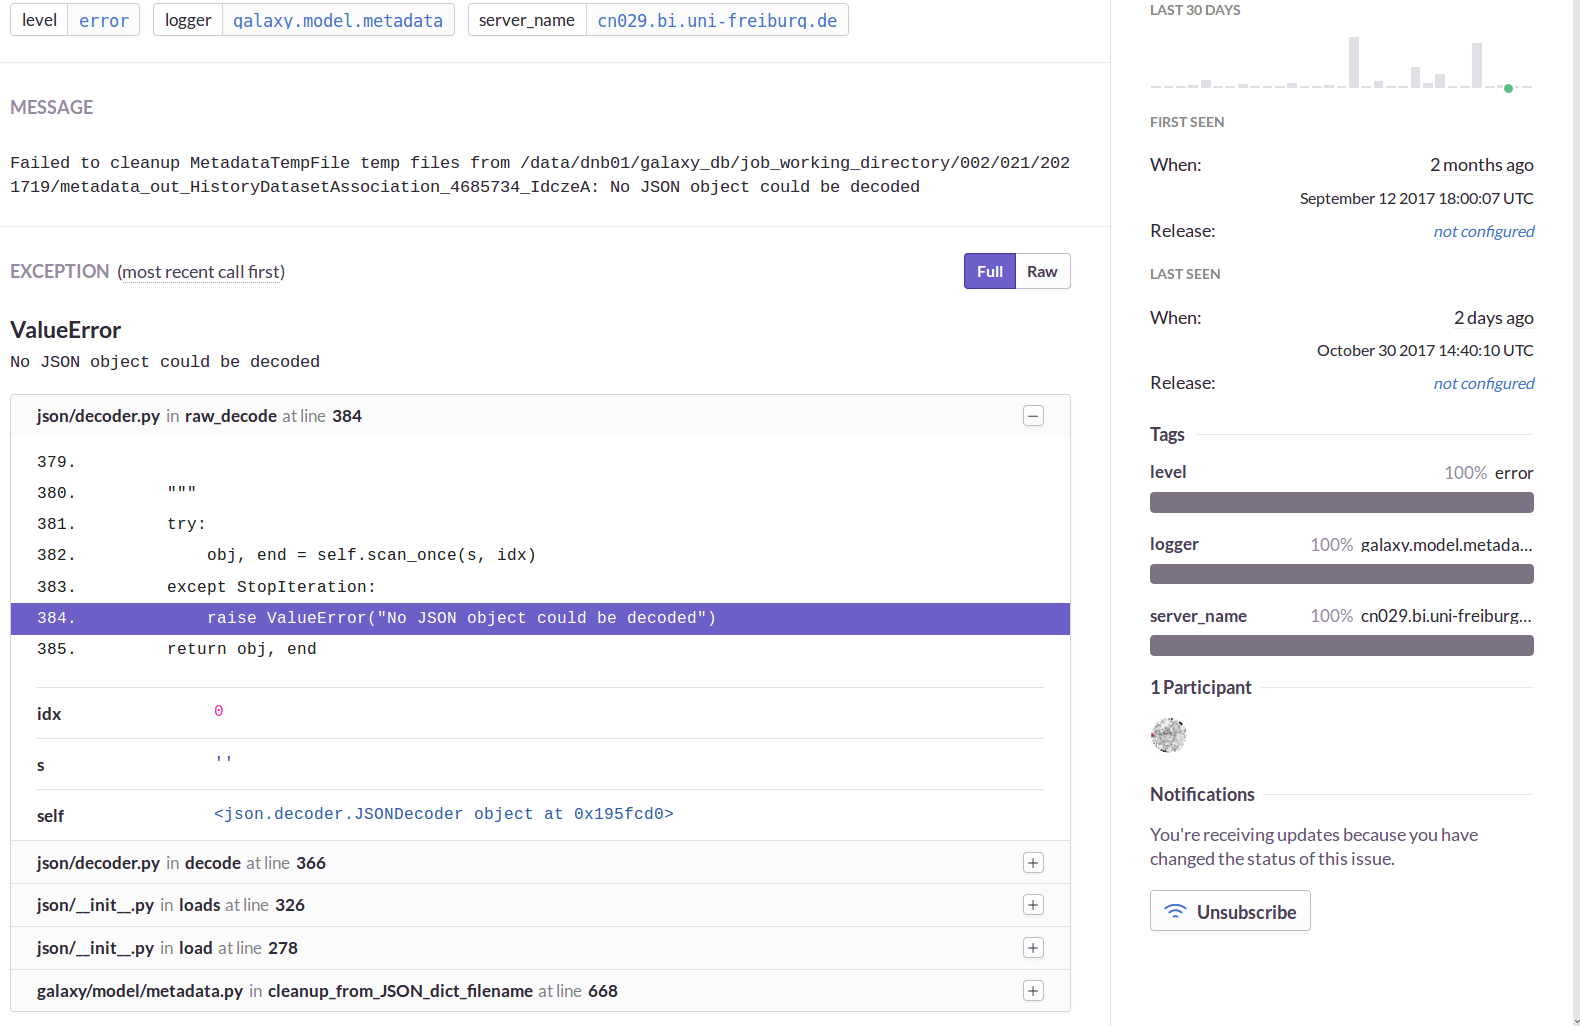
\includegraphics[height=\paperheight,width=\paperwidth]{sentry_2.png}}
		\setbeamertemplate{navigation symbols}{}
		\begin{frame}[plain]
		\end{frame}
	}

	\begin{frame}{Jenkins}
		\begin{center}
			\emph{New UFR Service}
		\end{center}
		\begin{itemize}
			\item Like \textbf{Travis-CI} but different
			\item Runs in the bwCloud
			\item Useful if:
				\begin{itemize}
					\item Jobs need to run really long
					\item Code is extremely private/sensitive
					\item Jobs produce artifacts that must be stored and
						available to download (e.g. PDF for course slides)
				\end{itemize}
		\end{itemize}
	\end{frame}

	\begin{frame}{public-galaxy-servers}
		\begin{itemize}
			\item CSV file of public galaxy servers
			\item Simple script to contact server + record configuration
			\item Uptime badges! 
\includegraphics[height=1em]{Freiburg_Galaxy.svg.png}
			\item Cool maps!
		\end{itemize}
		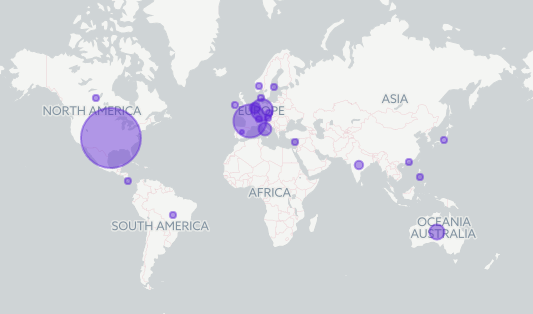
\includegraphics[width=\textwidth]{map.png}
	\end{frame}

	\begin{frame}{Galactic Radio Telescope}
		\begin{itemize}
			\item Part of Galaxy 17.09
			\item Efficiently collects basic metrics (job, state, runtime, input sizes) from participating Galaxies
			\item A later update will add more metrics
			\item Currently collecting from UFR Galaxy
			\item \url{https://telescope.galaxyproject.org}
		\end{itemize}
	\end{frame}

\subsection{Freiburg Galaxy}
	\begin{frame}{Job Conf Migration}
		\begin{itemize}
			\item Job configuration migrated from XML to python
			\item Job conf now under testing (Jenkins)
			\item Enables dynamically choosing where to send jobs
			\item Highlighted use case: Training-as-a-Service. Users in specific roles can be directed to dedicated VMs.
		\end{itemize}
	\end{frame}

	\begin{frame}{Upload + Metadata VMs}
		\begin{itemize}
			\item Leverages our bwCloud Condor Cluster
			\item ``Upload'' VMs only handle upload jobs, ``metadata'' VMs are similar.
			\item All uncompression of uploaded files is done off of \texttt{cn029}
			\item \emph{Fewer} random slow downs
		\end{itemize}
	\end{frame}

	\begin{frame}{yaml linting}
		\begin{itemize}
			\item \texttt{pykwalify} is great
			\item Use it.
				%TODO: image of schema
		\end{itemize}
		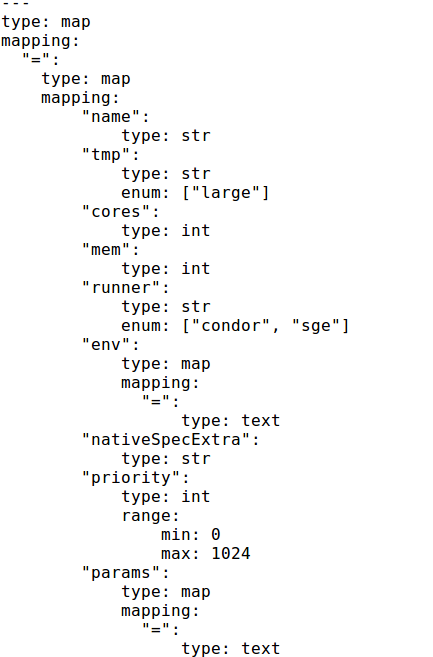
\includegraphics[height=0.8\textwidth]{pykwalify.png}
	\end{frame}

\subsection{Galaxy Project}
	\begin{frame}{Bug Reporting Plugins}
		\begin{itemize}
			\item Bug reporting as ``plugins''
			\item Plugins for: email, sentry, GitHub, influxdb, logfile
			\item Easy to develop new ones
			\item Control over automated submission without user interaction (e.g.~sentry vs email)
			\item \ghpr{galaxyproject}{galaxy}{4305}
		\end{itemize}
	\end{frame}

	\begin{frame}{Ansibilization of Galaxy Configuration}
		\begin{itemize}
			\item Major Galaxy configuration files now as some custom playbooks
			\item Not the entirety of galaxy
			\item Playbooks automatically run every hour
			\item GitHub enables reviewing + ``auditing'' of configuration changes
			\item \emph{Nearly} no more SSHing
		\end{itemize}
	\end{frame}

	\begin{frame}{Bigger Click Targets}
		\begin{itemize}
			\item \ghpr{galaxyproject}{galaxy}{4470}
			\item I hate small click targets
			\item Be the change you want to see in the world
		\end{itemize}
	\end{frame}

\subsection{Performance}
	\begin{frame}{Zerg Mode}
		\begin{itemize}
			\item \emph{Zero-downtime restarts of Galaxy}
			\item Configuration worked out by Nate Coraor (@natefoo)
			\item It is super effective!
			\item We annotate the restart events in Grafana if you are curious when it happens
		\end{itemize}
	\end{frame}

\subsection{Cloud}
	\begin{frame}{VGCN Images}
		\begin{itemize}
			\item Pre-configure Condor Master + Executor VM images
			\item Converted existing playbooks to reusable roles
			\item Integrated work from RZ for simplified build process
			\item Now regularly building + deploying images
		\end{itemize}
	\end{frame}

	\begin{frame}{VGCN Infrastructure}
		\begin{itemize}
			\item Regularly deploying new images sucked
			\item Rolling restarts are necessary
			\item Infrastructure-as-code (e.g. Terraform/CloudFormation/Heat)
		\end{itemize}
		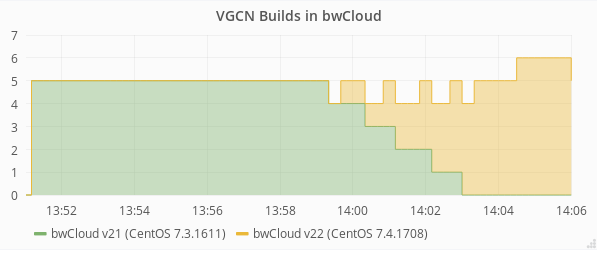
\includegraphics[width=\textwidth]{vgcn.png}
	\end{frame}

	\begin{frame}{bwCloud}
		\begin{itemize}
			\item Temporary maintainer
			\item Full time employee replaces me (yay!)
			\item No major improvements made, some networking issues triaged and bandaids applied around libvirtd
		\end{itemize}
	\end{frame}

\subsection{Security}

	\begin{frame}{Galaxy subprocess hardening}
		\begin{itemize}
			\item \ghpr{galaxyproject}{galaxy}{4604}
			\item \textbf{BAD}\\ \texttt{subprocess.call("ls /some/path", shell=True)}
			\item \textbf{GOOD}\\ \texttt{subprocess.call(["ls", "/some/path"])}
			\item Missed some \texttt{:(}
		\end{itemize}
	\end{frame}

	\begin{frame}{Reaching the promised LAN}
		\begin{itemize}
			\item \ghpr{galaxyproject}{galaxy}{4289}
			\item Galaxy's upload lets you paste in URLs
			\item Even URLs inside your super secure network (e.g.~\texttt{http://192.168.0.1:8080})
			\item Galaxy can be used to probe infrastructure and possibly download restricted material
			\item Now administrators must whitelist local network resources which should be accessible.
		\end{itemize}
	\end{frame}

	\begin{frame}{Security Repo for Galaxyproject}
		\begin{itemize}
			\item Tracking security issues in emails is not sensible
			\item We now have a git repo for this
			\item Testing setup is WIP
		\end{itemize}
	\end{frame}


\section[Ongoing]{Ongoing Projects}
\begin{frame}{Ongoing Projects}
\end{frame}

\subsection[FR Galaxy]{\texttt{usegalaxy.eu}}

	\begin{frame}{usegalaxy.eu rollout}
		Done:
		\begin{itemize}
			\item Many uptime and performance enhancements in place
			\item Monitoring continues to help identify issues
		\end{itemize}
		\ \\[0.5cm]
		TODO:
		\begin{itemize}
			\item Logo
			\item Branding things (UFR downplayed, usegalaxy.eu everywhere)
			\item English and grammar checks of all written materials
			\item Terms of Service (SLA, SLO) + Privacy Policy
			\item Communications Materials
			\item User-facing mailing list, plan out mails
		\end{itemize}
	\end{frame}

	\begin{frame}{Apollo}
		Background:
		\begin{itemize}
			\item We'll be deploying the Apollo Genome Browser alongside \texttt{usegalaxy.eu}
			\item Apollo has horrifying performance in some parts
			\item UI is miserable
			\item Underlying code is not easily fixed
		\end{itemize}
		\ \\[0.5cm]
		TODO:
		\begin{itemize}
			\item Working on splitting apart frontend + backend
			\item Collaborating with some other ``big'' apollo-galaxy sites
		\end{itemize}
	\end{frame}

	\begin{frame}{JBrowe Chat Plugin}
		Background:
		\begin{itemize}
			\item Apollo is great for collaborative, real-time editing
			\item \ldots{}but it feels very lonely since you cannot communicate
		\end{itemize}
		\ \\[0.5cm]
		Done:
		\begin{itemize}
			\item Proof-of-concept implementation works OK
		\end{itemize}
		\ \\[0.5cm]
		TODO:
		\begin{itemize}
			\item Needs more authentication options
			\item Needs archiving / chat log database
		\end{itemize}
	\end{frame}

	\begin{frame}{Production Services}
		Background:
		\begin{itemize}
			\item Increasing number services that become slowly critical
			\item SLAs? SLOs?
		\end{itemize}
		\ \\[0.5cm]
		Done:
		\begin{itemize}
			\item Ansible roles for deploying infrastructure (Grafana, InfluxDB, Sentry, public-galaxy-servers)
		\end{itemize}
		\ \\[0.5cm]
		TODO:
		\begin{itemize}
			\item SLO: \emph{Must} be able to be redeployed quickly ($<$\SI{10}{\minute})
			\item Backups
		\end{itemize}
	\end{frame}

	\begin{frame}{Advanced Job Conf}
		Background:
		\begin{itemize}
			\item ``New'' job conf is nice
			\item But can only be reconfigured by restarting handlers and waiting \SIrange{5}{10}{\minute}
		\end{itemize}
		\ \\[0.5cm]
		TODO:
		\begin{itemize}
			\item Force it into a secondary process which can be re-deployed with zero downtime
			\item Need to choose a method + test  (unix sockets, load balanced web service, \texttt{SO\_REUSEPORT}, etc.)
			\item SLO: $\leq\frac{1}{100.000}$ jobs dropped in networked version of the job destination service
		\end{itemize}
	\end{frame}

	\begin{frame}{Lecture Material Compilation + Archiving}
		\begin{itemize}
			\item Jenkins is now building NGS\_lectures as an example
			\item ``Reference'' build platform, everyone can compare results to
				it (especially for people with custom \LaTeX styles)
			\item Can serve + archive PDFs (forever?)
			\item Need to define artefact retention policy
			\item Need to apply to more projects
		\end{itemize}
	\end{frame}

	\begin{frame}{User Filters}
		Background:
		\begin{itemize}
			\item Too many tools in the toolbox
			\item Too few are relevant to specific users
			\item With user toolbox filters users can ``build'' their own toolbox
		\end{itemize}
		\ \\[0.5cm]
		TODO:
		\begin{itemize}
			\item Currently broken, will be fixed real soon now\texttrademark
		\end{itemize}
	\end{frame}

\subsection{Galaxy Project}

	\begin{frame}{pg\_tools}
		Background:
		\begin{itemize}
			\item (Re)discovered script \texttt{pglite}
			\item Will provide \emph{real} PostgreSQL databases during tool execution
			\item Useful for chemiinformatics + genome annotation
		\end{itemize}
		\ \\[0.5cm]
		Done:
		\begin{itemize}
			\item First set of tools being built
			\item Datatypes in Galaxy
		\end{itemize}
		\ \\[0.5cm]
		TODO:
		\begin{itemize}
			\item GMOD tool suite
			\item chado-schema-builder brought back to life
		\end{itemize}
	\end{frame}

	\begin{frame}{Mirroring Galaxy Repos}
		Background:
		\begin{itemize}
			\item Some devs worry: ``What if GitHub goes away?''
			\item Plan is to mirror all of galaxyproject's repos
		\end{itemize}
		\ \\[0.5cm]
		Done:
		\begin{itemize}
			\item Simple mirror of Galaxy codebase
		\end{itemize}
		\ \\[0.5cm]
		TODO:
		\begin{itemize}
			\item Mirror all other repos
			\item Update mirrors regularly (i.e. Jenkins job)
			\item Recently discovered \texttt{git-appraise}. Should permit archiving PRs + discussion (+ issues?) all within portable git repo.
		\end{itemize}
	\end{frame}

\subsection{Performance}
\subsection{Cloud}

	\begin{frame}{deNBI Cloud}
		\begin{itemize}
			\item Adding Elixir AAI authentication to deNBI Cloud @ Freiburg
			\item Unlike any other cloud, so we have special issues
			\item \texttt{:(}
		\end{itemize}
	\end{frame}

	\begin{frame}{Automating VGCN Image Building}
		Background:
		\begin{itemize}
			\item Building VGCN images by hand is time consuming
			\item Builds are quite reliable, unlikely to produce a broken VM
			\item So let's make Jenkins build them on VGCN playbook changes
		\end{itemize}
		\ \\[0.5cm]
		TODO:
		\begin{itemize}
			\item Builds in bwCloud time out when Jenkins runs them
			\item But they'll build fine in SJ's ``imager'' cloud VM
			\item ???
		\end{itemize}
	\end{frame}

\subsection{Security}

	\begin{frame}{CSP}
		Background:
		\begin{itemize}
			\item CSP helps prevent huge swaths of security issues
			\item Can prevent browsers from executing unexpected scripts, CSS, media, frames, etc.
		\end{itemize}
		\ \\[0.5cm]
		Done:
		\begin{itemize}
			\item Currently in ``reporting'' mode, collecting any infractions
		\end{itemize}
		\ \\[0.5cm]
		TODO:
		\begin{itemize}
			\item Need to analyze infractions, identify real issues (vs noise)
			\item Need to cleanup galaxy, removing inlined styles, scripts
			\item Will move to ``enforcing'' mode after issues are patched
		\end{itemize}
	\end{frame}

	\begin{frame}{Cron jobs logged to Jenkins}
		Background:
		\begin{itemize}
			\item Ansibilization lets us discover all manner of hidden jobs
			\item Let's push the logs to a central location for auditing
			\item Jenkins can ``monitor'' external jobs
			\item Public visibility $\Rightarrow$ forced accountability
		\end{itemize}
		\ \\[0.5cm]
		Done:
		\begin{itemize}
			\item All cron tasks from \texttt{galaxy@cn029}
		\end{itemize}
		\ \\[0.5cm]
		TODO:
		\begin{itemize}
			\item Identify cron jobs on other hosts, VMs, etc.
		\end{itemize}
	\end{frame}


\section[Upcoming]{Upcoming Projects}
\begin{frame}{Upcoming Projects}
	Still in planning phase
\end{frame}

\subsection{Monitoring}

	\begin{frame}{GRT Analysis Suite}
		Question: What is in the GRT data? \\[0.6cm]
		Proposed Solution:
		\begin{itemize}
			\item Deploy Jupyter / an web-based SQL query suite with access to GRT data.
			\item No real plan for making it useful, but it'd be shiny
			\item Want to encourage analysis of public GRT data
		\end{itemize}
	\end{frame}

	\begin{frame}{Testing Workflow execution}
		Question: Is Galaxy working as expected? \\[0.6cm]
		Proposed Solution:
		\begin{itemize}
			\item Regular, automated testing of our Galaxy installation
			\item Commonly executed workflows will give good idea
			\item Can cover jobs going to condor + sge + odd configuration we might have
		\end{itemize}
	\end{frame}

	\begin{frame}{More monitoring}
		Question: Why is everything still slow? \\[0.6cm]
		Proposed Solution:
		\begin{itemize}
			\item Upload jobs should be timed (time to upload, job execution, green history element)
			\item More job timings available in the database
			\item Need to track all of this
			\item In general, are things getting better or worse for users?
			\item Is user-facing infra more or less reliable?
		\end{itemize}
	\end{frame}

\subsection{Freiburg Galaxy}

\subsection{Galaxy Project}

	\begin{frame}{GIS}
		Question: How can I analyse geographic data in Galaxy? \\[0.6cm]
		Proposed Solution:
		\begin{itemize}
			\item French team wants to work on this
			\item GIS data is super fun, we can work with some interesting datasets
			\item Lots of room to build stuff people will love
		\end{itemize}
	\end{frame}

\subsection{Performance}

\subsection{Cloud}

\subsection{Security}

	\begin{frame}{Galaxy OAuth2}
		Question: How can I grant partial access to my account to a third party without violating every security policy ever? \\[0.6cm]
		Proposed Solution:
		\begin{itemize}
			\item Implement \emph{OAuth2} over the Galaxy API
			\item API keys with \emph{scopes} that can be granted
			\item Third parties can build things on top of Galaxy, new UIs, new (limited) tools
			\item Users feel safe granting privileges
		\end{itemize}
	\end{frame}

	\begin{frame}{User Generated Content}
		Question: How can admins be 100\% absolutely sure that user generated content is safe? \\[0.6cm]
		Proposed Solution:
		\begin{itemize}
			\item Host user-content on a second domain (i.e. HTML render of datasets)
			\item Just like GitHub (\texttt{githubusercontent.com})
			\item Will allow us to ignore / disable whitelisting of ``safe'' tools
			\item Token-based access to datasets instead of cookie-based
		\end{itemize}
	\end{frame}

	\begin{frame}{Secrets Server}
		Question: How can we securely store user-supplied secrets in the safest way possible? \\[0.6cm]
		Proposed Solution:
		\begin{itemize}
			\item Galaxy should not be responsible for storing super secret secrets (e.g. API keys to third party services)
			\item Hashicorp's Secrets Server is \emph{literally built for this and only this}
			\item Integration paves way for tools with easier access to remote services (i.e. Apollo suite)
		\end{itemize}
	\end{frame}

	\begin{frame}{Medical / DFARS}
		Question: How can users with extreme data security requirements use Galaxy?\\ \ \\
		Proposed Solution:
		\begin{itemize}
			\item Allow users to mark datasets, libraries, entire histories as ``secure''
			\item Any datasets produced from these are also tagged ``secure'' and treated accordingly.
			\item For datasets marked as ``secure'':
				\begin{itemize}
					\item Must securely wipe (DoD standard 32-pass) datasets and temporary files
					\item Data must be encrypted in transit + at rest (requires Secrets Server)
				\end{itemize}
		\end{itemize}
	\end{frame}

	\begin{frame}{Caching Framework}
		Question: How can we keep Galaxy from re-building the same tools, the same JSON blobs \textit{ad nauseam}?\\[0.6cm]
		Proposed Solution:
		\begin{itemize}
			\item Provide a generic interface in codebase for caching data
			\item Provide methods for expiring the cache as needed
			\item Will support in-memory, on-disk, and networked caches (memcached)
			\item Will convert subset of slow computations to use new cache
		\end{itemize}
	\end{frame}
\end{document}
